\section{Introduction to Parallelism}
\label{sec:introduction to parallelism}
The goal of using GPGPUs is to solve computational problems, either faster or bigger than what was previously possible with CPUs.
Often a simple port of a piece of code, given it has a parallel nature, will resolve in a significant speed up (3x to 5x)~\cite{udacity}.
However, utilizing the software and hardware it is possible to go way beyond the initial speed up.
The principles of GPGPU programming when coding for efficiency is to maximize useful operations by minimizing memory bottlenecks and divergence that force waiting time amongst threads.

It is useful to abstract the optimisation to different levels as some optimisations might be more useful than others.

\begin{enumerate}
\item Picking good algorithms
\item Basic principles for efficiency
\item Architecture specific detailed optimisations
\item Micro optimisations
\end{enumerate}

The single most important element in optimisation is to pick an algorithm with strong asymptotic bounds.
Optimising insertion sort $\mathcal{O}(n^2)$ as opposed to merge sort $\mathcal{O}(n\log n)$ would make even a naive implementation of merge sort vastly superior to a very optimised version of insertion sort.
We will discuss algorithms specific for parallel coding in \cref{sec:software optimisations}

Further, when considering algorithms for parallel purposes, the parallelisability in an algorithm is of importance.
When designing algorithms we will view the computations as a directed acyclic graph (DAG).
This graph will have a set of computational steps linked together from top till bottom such as illustrated in \cref{fig:step and work}.

\begin{figure}[htb]
  \centering
  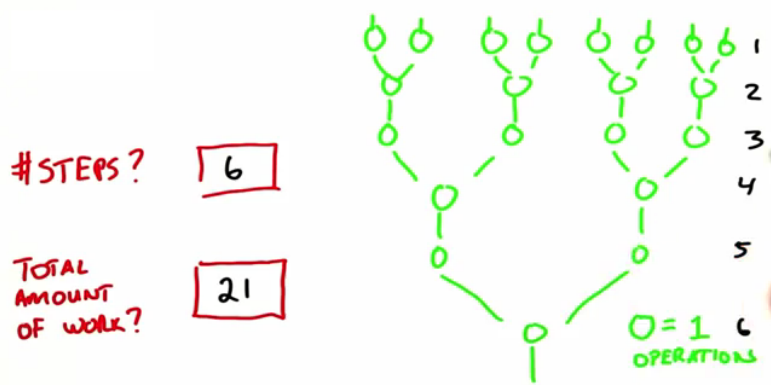
\includegraphics[width=.7\textwidth]{images/step-work.png}
  \caption{Calculating step and work size}
  \label{fig:step and work}
\end{figure}

The important aspect is the workload to step ratio. The workload decides the total amount of work nessesary for that specific algorithm whereas the step size determinez the amount of serial work in the algorithm.
For an algorithm to have a parallel nature the step size has to be relatively low compared to the workload.
When we describe the algorithms we have computed in the algorithmic section we will also describe the algorithms work load and step size.

Basic principles for efficieny is the second most important aspect.
Developing cache aware kernels that utilizes the cache efficiently is critical to reduce memory bottlenecks.
In \cref{sec:memory optimisations} we will provide tricks to optimize the memory transfers and utilize faster memory.

Architectural specific optimisation concerns utilizing the given architecture of a specific GPGPU's SM such as amount of threads per SM, L1 cache size for shared memoryetc.
In \cref{sec:hardware optimisations} we will consider how to utilize the GPGPU architecture when setting kernel parameters.

Micro level optimisation works at the bit-level, such as approximating the inverse of a square root with magic numbers.
We will not consider these types of optimisations on the GPGPU in this report as the gains are minimal compared with the other optimisations \cite{udacity}.
